\section{Measurements}
\label{sec:measurement}
In the following section we discuss the measurements that we performed as part of our study. We start out by measuring the kaudit buffer utilization and audit latency to highlight the pitfalls of naively enabling auditing on a RTS. We then adapt the audit system to real-time scheduling as described in Section~\ref{sec:sched} and measure the log maintenance overhead.

\subsection{Buffer Utilization}

\textbf{Experiment:}

 For measuring the utilization of the kaudit buffer, we periodically sampled the buffer state every 2 seconds using the audit command line utility \textit{auditctl}, while executing the ArduPilot application for 100K iterations. 

\textbf{Observations:} From Figure~\ref{fig:eval_backlog}, we see that for Linux Audit, the utilization of the kaudit buffer rises quickly in the beginning and remains close to 100\% for the majority of the running time, resulting in loss of audit messages.

\begin{figure}[t!]
    \centering
    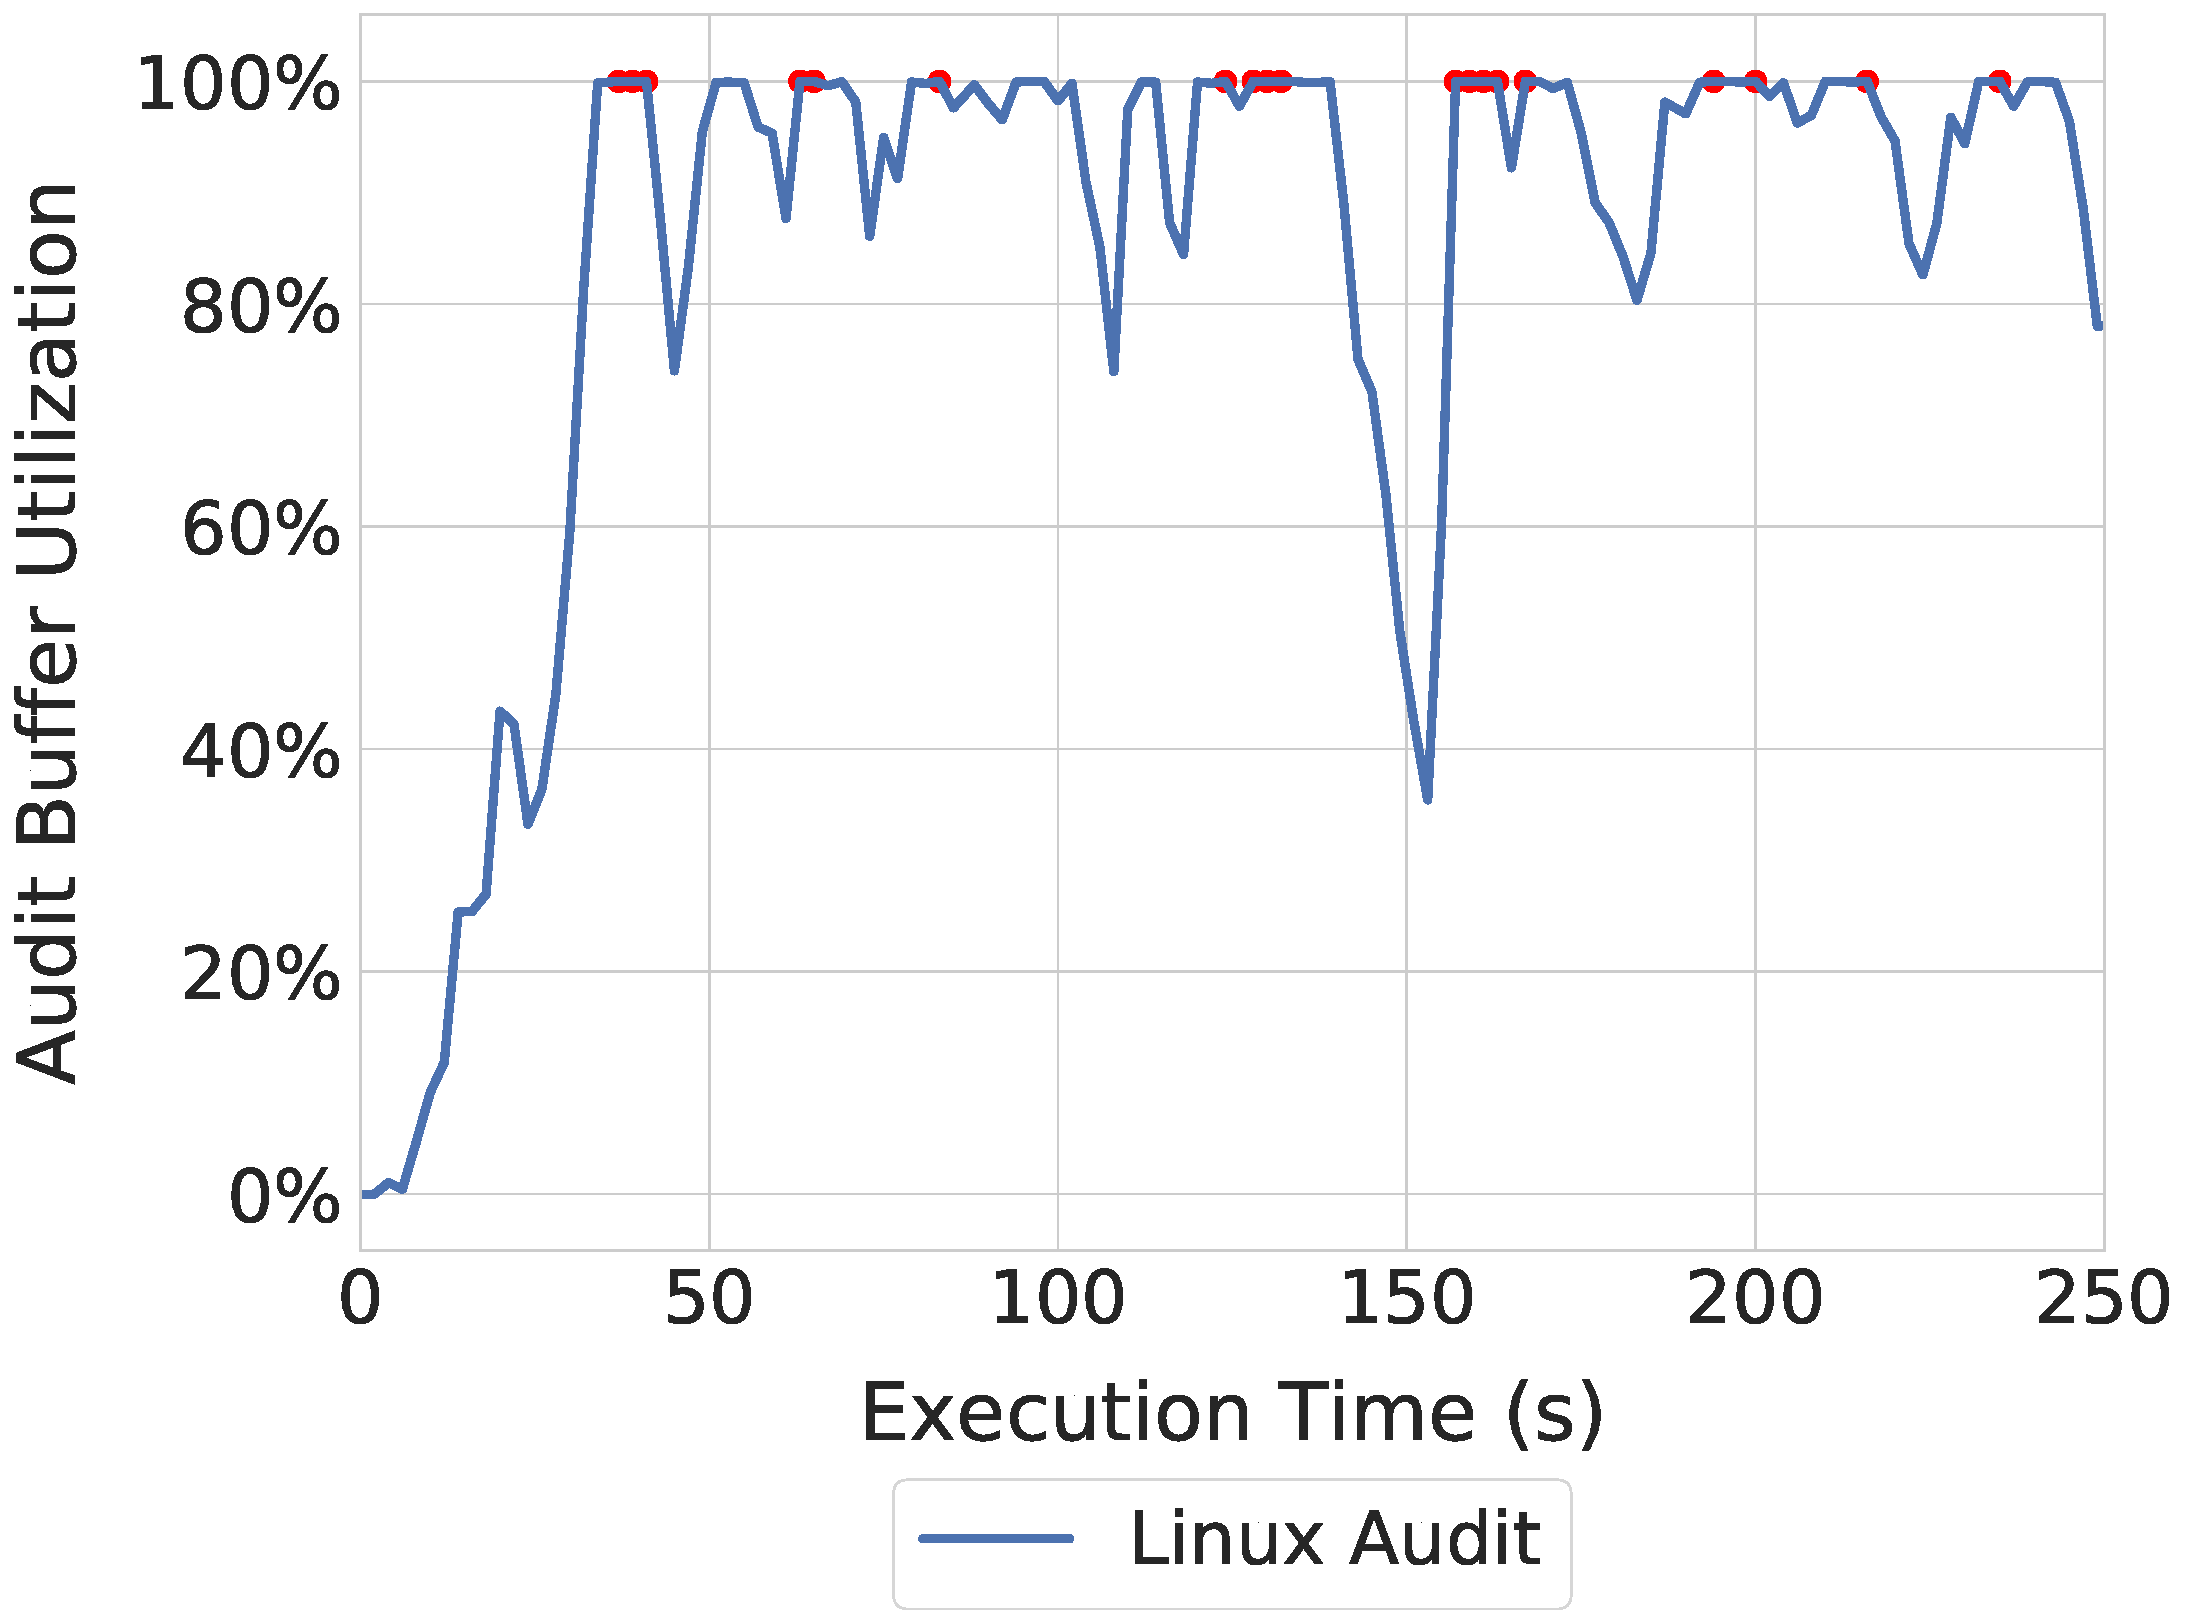
\includegraphics[width=0.9\linewidth,keepaspectratio,scale=0.9]{fig/backlog_over_time_hlight.pdf}
    \caption{\label{fig:eval_backlog}Kaudit buffer utilization over time for Linux Audit. Linux Audit's {\tt backlog} value was measured every 2 seconds during the execution of the application and plotted as a percentage of the max backlog limit.
    Additional red annotations signify all times when buffer utilization was 100\% and hence audit events might be lost. At these points Linux Audit performance is actually worse than depicted, but was constrained by the allotted buffer space.}    
\end{figure} 

\textbf{Discussion:}
When the kaudit buffer is full, new audit messages are lost; hence, to ensure that suspicious events are recorded, it is essential that \textit{the buffer is never full}.
The variations that we see in the plots can be attributed to the scheduling of the non-real-time \textit{kauditd} thread that is responsible for sending the outstanding audit messages to user-space for retention on disk. We observe that the backlog builds with time when \textit{kauditd} isn't scheduled and drops sharply when \textit{kauditd} eventually gets CPU time. 

As \textit{kauditd} is a non-real-time thread running with no priority, it contends with multiple background processes for CPU time resulting in high buildup of messages in the kaudit buffer. Reducing the pressure of incoming audit messages using a kernel based log reduction scheme like KCAL \cite{Ma2018} or increasing the rate of draining the kaudit buffer could be suitable approaches to ensure lossless auditing in resource constrained systems.

\subsection{Audit Latency}
\textbf{Experiment:}



For measuring the amount of time each audit message spends in the audit subsystem, the ArduPilot application was executed over 10K iterations and the audit latency was computed using the commit time and the creation time of each audit message obtained from the audit log file. The non-real-time \textit{kauditd} and \textit{auditd} threads are assigned defaults nice value of 0 and -4 respectively.

\textbf{Observations:} From Figure~\ref{fig:eval_latency}, we see that the audit latencies across 140k audit messages has a very wide range from 130 microseconds to 1.38 seconds with a median of \~740 ms. 

\begin{figure}[t!]
    \centering
    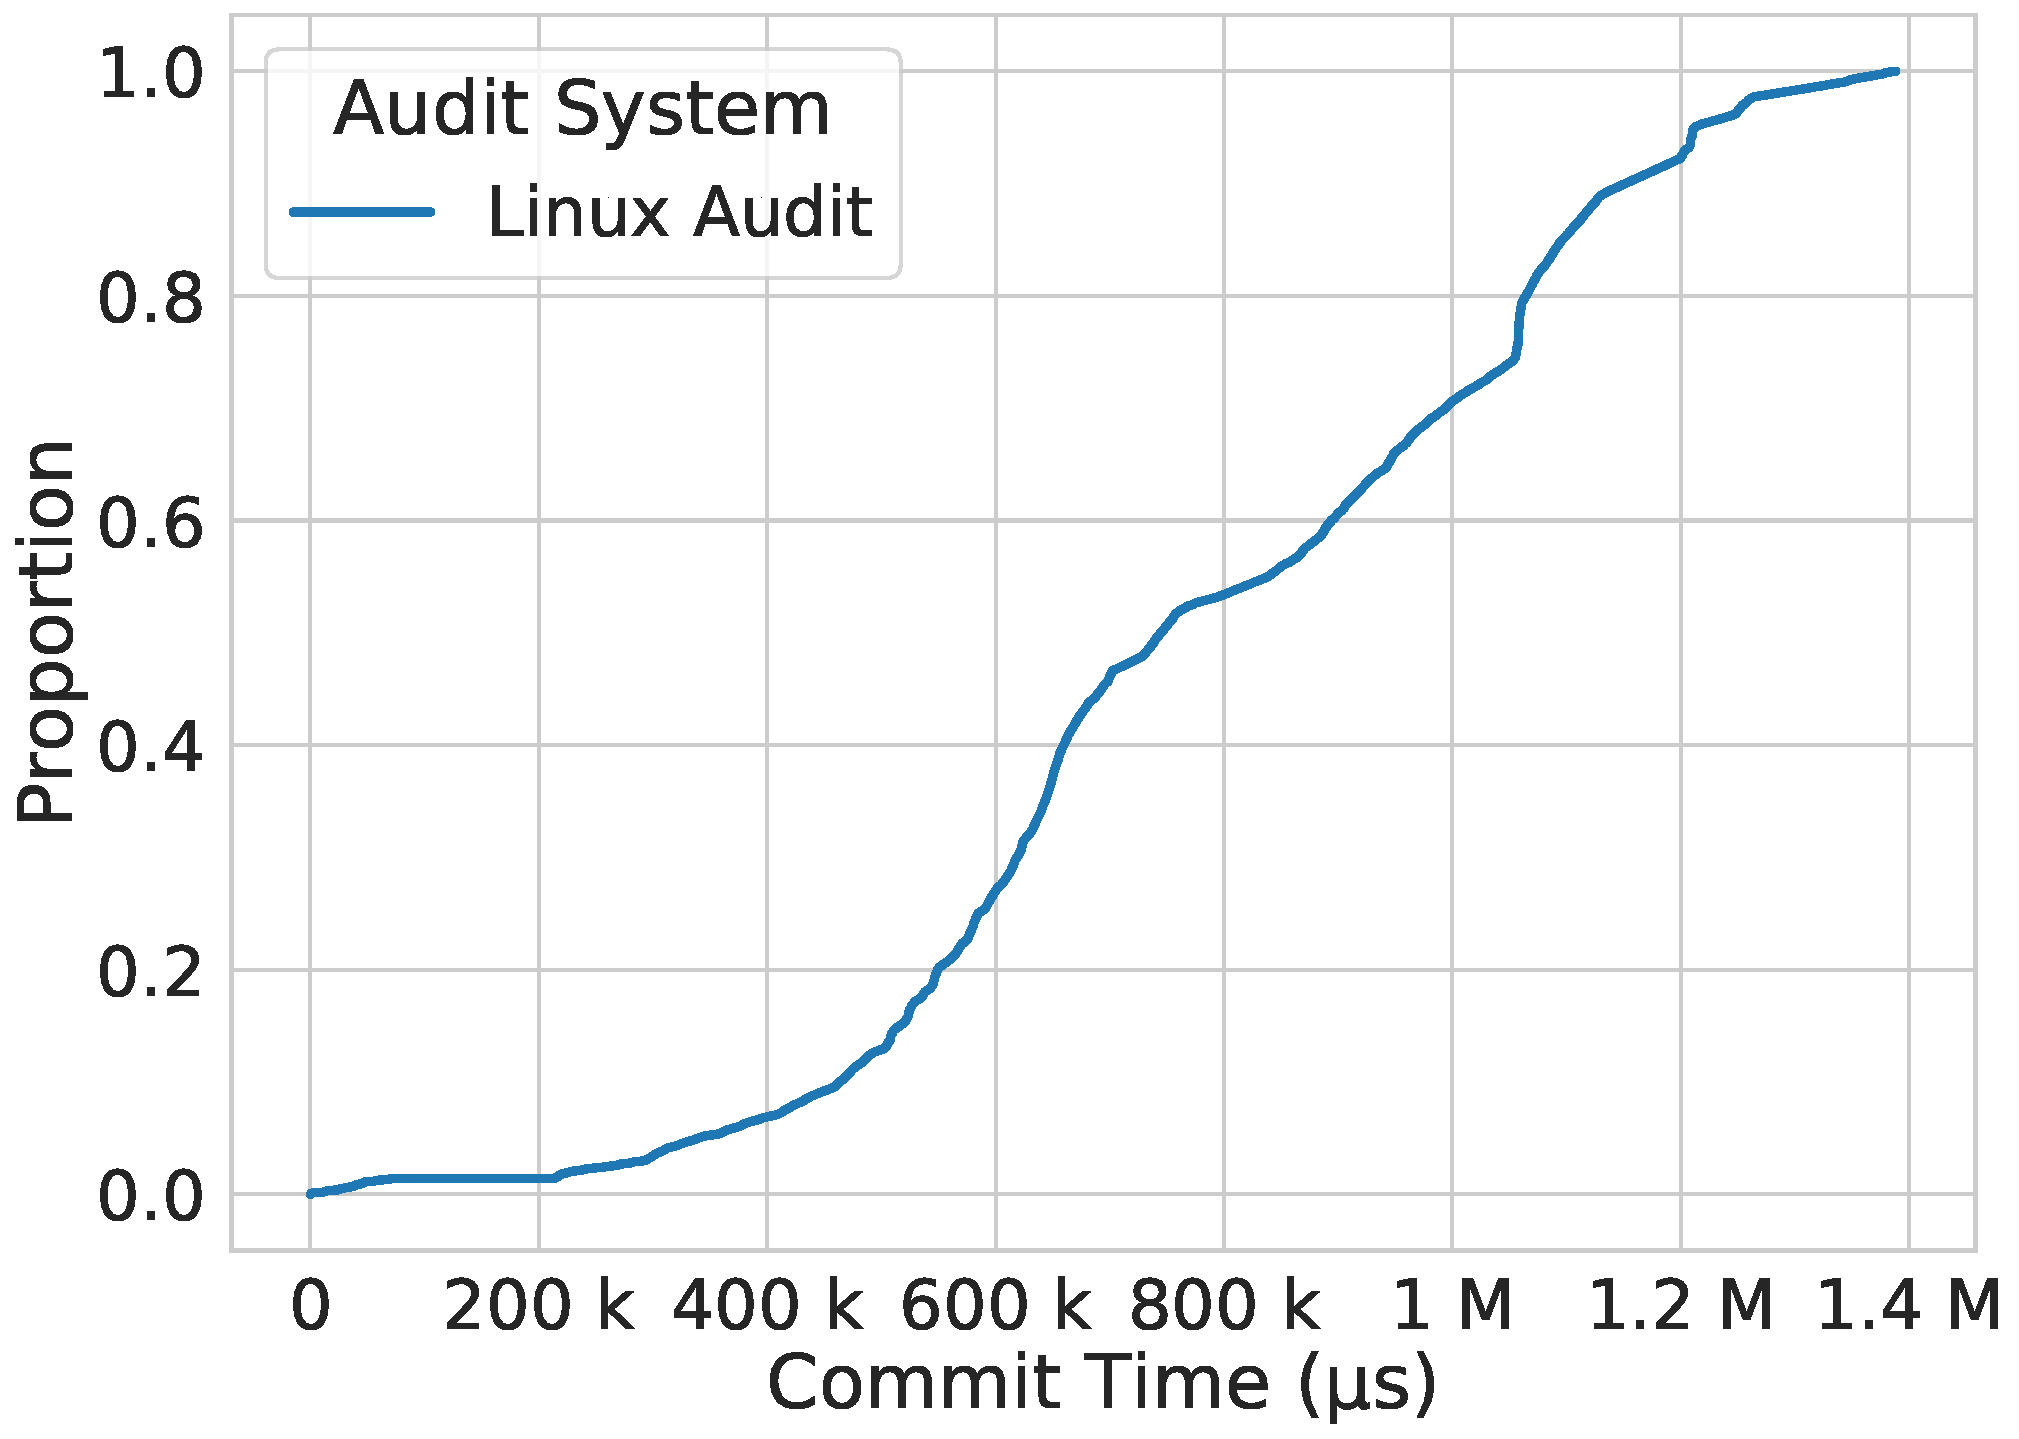
\includegraphics[width=0.9\linewidth,keepaspectratio,scale=0.9]{fig/Commit_latencies_cdf.pdf}
    \caption{\label{fig:eval_latency}Audit commit latencies over time for Linux Audit plotted as a Cumulative Distribution Function (CDF). The experiment measures the time between the generation of an audit message and before the message is written to disk in user space by the \textit{auditd} thread. For a chosen commit time \textit{t} on the x-axis, the y-axis shows the fraction of the total messages that encountered delay of less than \textit{t} microseconds.}
\end{figure}

\textbf{Discussion:} 
The wide range of audit latencies points us to the fact that vanilla Linux Audit maybe a poor choice for real time systems, which typically demand predictable and tightly bound temporal performance guarantees. The low observed minimum audit latency suggests that the implementation of the audit subsystem itself may not entirely to blame for the high \textit{kauditd} buffer utilization and reinforces our earlier observation that scheduling of audit threads is the primary reason for the long tail in audit latencies.

As the audit threads execute at lower non-real-time priorities, they rely on adequate application slack time to complete execution. With the introduction of synchronous and asynchronous overheads of auditing, the effective slack time reduces further taking away CPU time from the audit subsystem. Reliably accounting for these auditing overheads and increasing priorities of audit threads could help design a schedulable audited RT system and reign in the tail audit latencies.

\subsection{Log Maintenance Overhead}
\textbf{Experiment:}


For measuring the amount of time required to process a single audit message by the asynchronous audit threads, we ran a micro benchmark application that consisted of 10 \textit{getpid} system calls and observed the intervals at which audit messages were written to disk over 10 runs. In the RT+PIN scenario, we replicate the scenario described in Case II of Section~\ref{sec:sched} by assigning both kernel threads a low real time priority. We further pinned the \textit{auditd} thread to core 2 on the machine. As \textit{kauditd} is a kernel thread, we weren't able to pin the thread to a fixed core on the system, instead relying on its real time priority to ensure that it ran ahead of any background process. Whereas in the PRI scenario, the priorities of the audit threads were increased by modifying their nice values, which resembles the default configuration of the audit subsystem — where only the user space daemon gets a priority boost.

\begin{figure}[t!]
    \centering
    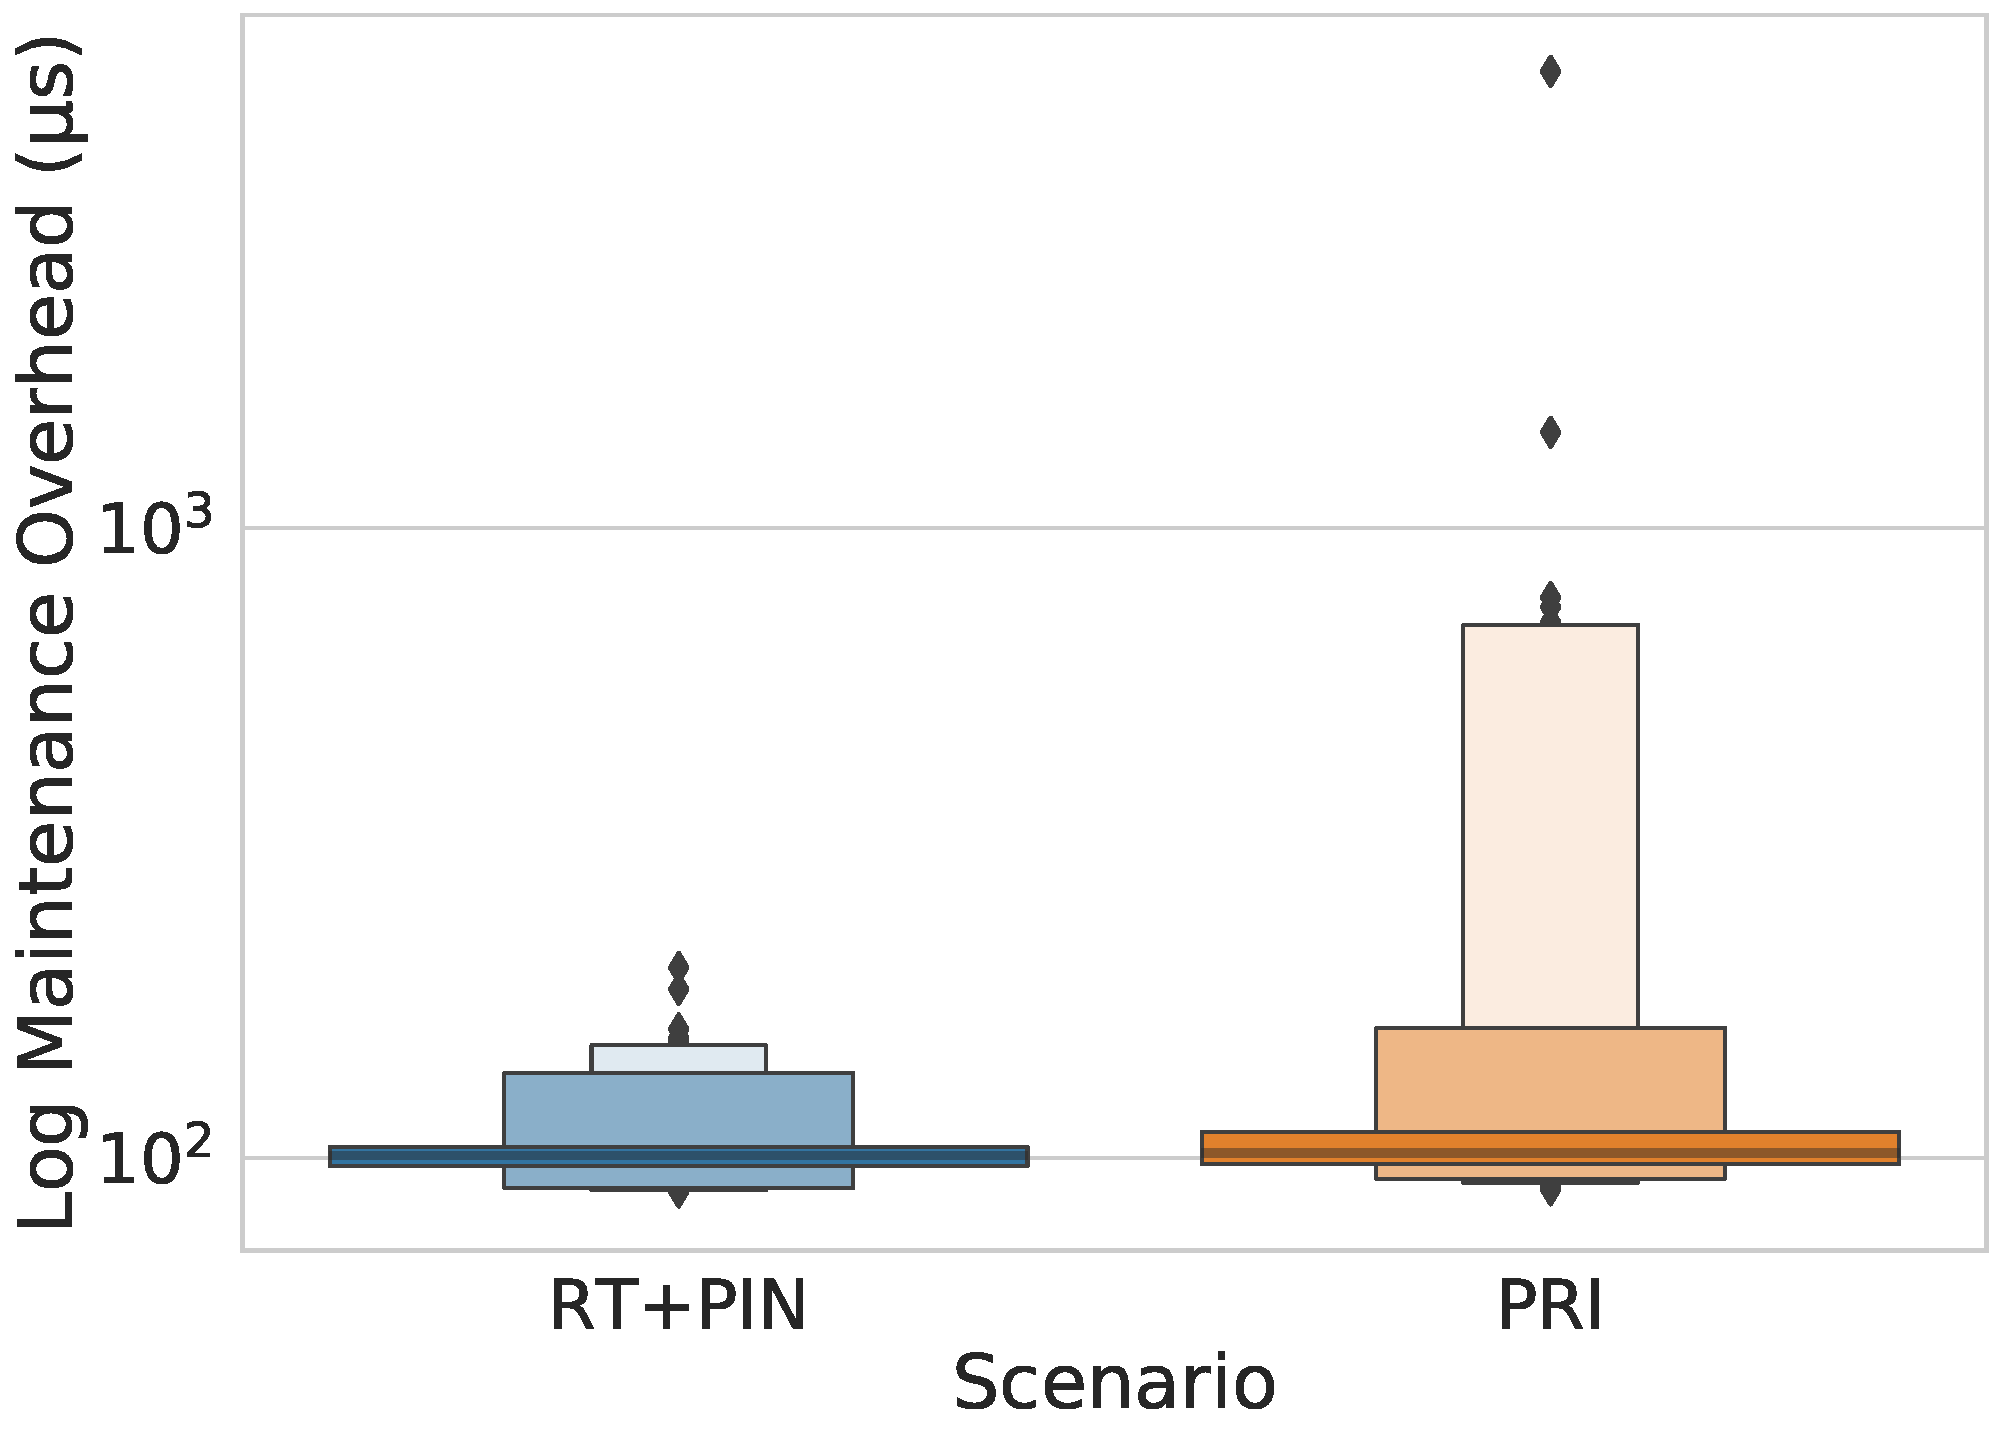
\includegraphics[width=0.9\linewidth,keepaspectratio,scale=0.9]{fig/Throughput.pdf}
    \caption{\label{fig:eval_throughput}Log maintenance overhead in microseconds over different system configurations. For \textit{RT+PIN}, we assign low real time priorities to the audit threads and pin \textit{auditd} to core 2. For \textit{PRI} we assign low non-real time priorities to both audit threads, similar to the default configuration for the audit system.}
\end{figure}

\textbf{Observations:} From Figure~\ref{fig:eval_throughput}, we observe that for the PRI case, the log maintenance overhead varies from 88 $\mu$s to 5ms. Introducing real time priorities and core pinning reduces the variance in measurements and reduces the maximum overhead to 200 $\mu$s.
 
\textbf{Discussion:} %\todo[inline]{Wrap up discussion — fairly obvious that low priority + core pinning would have worked — reduces time wasted in moving task around and moves it above background task, ensures CPU time —  need to add a core to ensure enough CPU time for the buffer — that could be reasonable as it can be factored in during the design phase itself — having an upper bound on the audit throughput helps plan for schedulability}
The order of magnitude reduction in maintenance overhead corresponding to a system call event highlights the competitions for processor time in the system. Assigning a low real time priority to both threads and pinning the user space \textit{auditd} thread to a core, reduces this competition and allows the audit subsystem to occupy all the slack time in the system, thereby eliminating delays due to preemption and context switching.\\
A naive approach to ensure lossless auditing could be to introduce an additional core in the system dedicated to auditing tasks. If the real time application has enough slack to process audit logs generated in a hyper period, we can assign a low real-time priority to both audit threads to avoid additional hardware resources. The estimates for audit processing times obtained from the experiment can help arrive at a lower bound on the required slack in the system. For real time systems which undergo rigorous schedulability analysis before deployment, choosing either approach can be a conscious decision based on the timing profile of the system.

\subsection{Summary of Results}
%\todo[inline]{Summarize takeaways — timing comes in handy to understand resource allocation — we can understand if log reduction is required once we are maxed out on our resource allocation.}
Based on the measurements, we find that naively enabling auditing on a real-time system can have serious implications on the completeness of audit logs. Log reduction techniques can help us ensure completeness of audit logs and accounting for synchronous and asynchronous overheads introduced by auditing frameworks can help reliably schedule real-time tasks. %scan help us auditing system calls can also impact schedulability of real-time tasks.% and a synergistic co-design of the audit framework and hardware might be required to ensure lossless auditing in a real-time system.